\documentclass[11pt]{beamer}
\usepackage[utf8]{inputenc}
\usepackage[T1]{fontenc}
\usepackage{amsmath}
\usepackage{amsfonts}
\usepackage{amssymb}
\usepackage{graphicx}
\usepackage{tikz}
\usepackage{booktabs}
\usepackage{color}
\usetheme{Dresden}


% images
\graphicspath{ {D:/Users/saketh/Documents/GitHub/OrderRoutingAndPFOF/exhibits/} }

% sig stars
\def\sym#1{\ifmmode^{#1}\else\(^{#1}\)\fi}

% wideness
\newcommand\Wider[2][3em]{%
	\makebox[\linewidth][c]{%
		\begin{minipage}{\dimexpr\textwidth+#1\relax}
			\raggedright#2
		\end{minipage}%
	}%
}

% footnotes
\setbeamerfont{footnote}{size=\scriptsize}


\begin{document}
	\author{Saketh Aleti \\ Advisor: Professor Bruce Mizrach}
	\title{The Effect of Payment for Order Flow on Broker Order Routing}
	%\subtitle{}
	%\logo{}
	%\institute{Advisor: Professor Bruce Mizrach}
	%\date{February 22}
	\subject{}
	%\setbeamercovered{transparent}
	%\setbeamertemplate{navigation symbols}{}
	\begin{frame}[plain]
	\maketitle
\end{frame}

\section{Introduction}

\begin{frame}
\frametitle{Research Question}

	\begin{block}
		{How does payment for order flow affect broker order routing?}	
	\end{block}

	\centerline{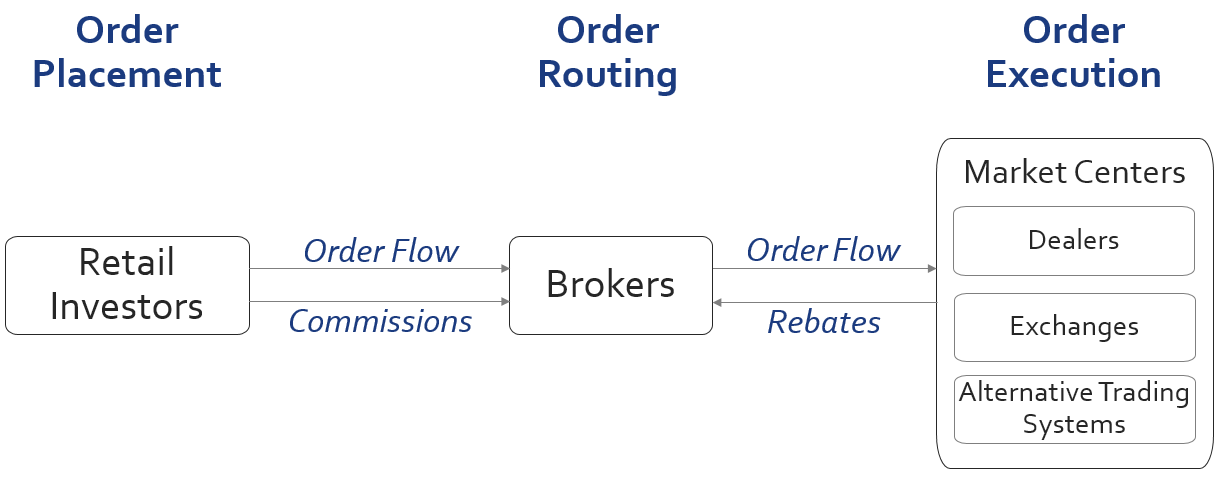
\includegraphics[scale=0.3]{order_routing_diagram.PNG}}
	\vspace{-1em}
	\begin{itemize}
		\item Payment for Order Flow (POF)
		\begin{itemize}
			\item Rebates given to brokers by market centers for order flow
			\item Usually a bit less than $\$0.03$ per 100 shares
		\end{itemize}
	\end{itemize}

\end{frame}

\begin{frame}
\frametitle{Motivation and Approach}

\begin{itemize}
	\setlength\itemsep{1em}
	\item Does retail investor welfare suffer from the presence of POF?
	
	\item SEC renounces negative statements about POF's effect on order routing  (Exchange Act of 1934 - Rule 11Ac1-5)

	\item Basic idea: Study differences between POF brokers and Non-POF brokers
	\begin{itemize}
		\setlength\itemsep{0.5em}
		\item Suppose a market center improves its execution speeds
		\item Non-POF brokers would reroute $\Delta\%$ of their orders to them
		\item POF brokers would reroute less than $\Delta\%$, because they also consider rebates
	\end{itemize}

\end{itemize}

\end{frame}

\begin{frame}

	\begin{block}{Hypothesis}
		\begin{itemize}
			\item Brokers who accept POF are less reactive to changes in execution quality than brokers who do not
			\begin{itemize}
				\setlength\itemsep{0.4em}
				\vspace{0.25em}
				\item Execution quality: price improvement and execution speed
				\item Theory $\implies $ brokers cannot simultaneously consider rebates as an objective while maximizing execution quality \footnote{Dennert (1993), Duta and Madhavan (1997), Parlour and Rajan (2001), Cimon (2016), Maglaras, Moallemi, and Zheng (2015)}			
				\item Empirics $\implies$ broker order routing for \textit{limit} orders was negatively impacted by payment for order flow \footnote{Battalio, Shkilko, and Van Ness (2016), Battalio, Corwin, and Jennings (2016)}
			\end{itemize}
		\end{itemize}
	\end{block}


\end{frame}


\section{Methodology}

\begin{frame}
\frametitle{Data}

\begin{block}
	{606 Disclosures}
	\begin{itemize}
		\item Broker reports of order routing data 
		\item \textbf{Market share}: \% of orders routed to a market center
		\item \textit{Most } of the time, brokers disclose the influence of POF
	\end{itemize}
\end{block}

\begin{block}
	{605 Disclosures}
	\begin{itemize}
		\item Market Center reports of execution statistics 
		\item \textbf{Execution quality} by stock, order type, and size
	\end{itemize}
\end{block}

\end{frame}


\begin{frame}
\frametitle{Descriptive Statistics - Price Improvement}

\fontsize{6pt}{7}\selectfont

\center{\includegraphics[scale=0.5]{descriptive/primp_expamt.pdf}}

\end{frame}


\begin{frame}
\frametitle{Descriptive Statistics - Execution Speed}

\fontsize{6pt}{7}\selectfont

\center{\includegraphics[scale=0.5]{descriptive/primp_avgt.pdf}}
\end{frame}



\begin{frame}
\frametitle{Methodology}


	\begin{itemize}
		\setlength\itemsep{0.5em}
		\item 	$	Y_{i, j, k,  t} \,=\, \alpha_{i,j} \,+\,  X_{j, k, t} \cdot \beta \,+\,  (D_i \cdot X_{j, k, t}) \cdot \gamma\, +  \varepsilon_{i, j, t}$
		\begin{itemize}
			\setlength\itemsep{0.5em}
			\vspace{0.25em}
			\item $Y_{i, j, k,  t}$ = \% of Orders Routed by Broker $i$ to Market Center $j$
			\item $X$ = Execution Quality
			\item $D_i$ = Indicator for POF
		\end{itemize}
		\vspace{0.5em}
		\item Parametric Approach with Tobit and OLS 
		\item Semiparametric Approach with SLS (Ichimura, 1993)
		\begin{itemize}
			\vspace{0.25em}
			\setlength\itemsep{0.5em}
			\item $Y_{i, j, k, t} = f(X_{j, k, t} \cdot \beta) +  v_{i,j,t}$
			\item Gaussian kernel
		\end{itemize}
	\end{itemize}


\end{frame}




\section{Results}

\subsection{Regressions}

\begin{frame}
\fontsize{6pt}{7}\selectfont
\Wider[5em]{
\begin{table}[!htbp] \centering 
	\caption{Tobit Regression Results} 
	\label{} 
	\begin{tabular}{@{\extracolsep{0.5em}}lcccc} 
		\\[-5ex]\hline  
		\hline \\[-1.8ex]  
		& \multicolumn{4}{c}{\textit{Dependent variable: Market Share}} \\  
		\cline{2-5}  
		\\[-1.8ex] & (1) & (2) & (3) & (4)\\  
		\hline \\[-1.8ex]  
		Percent of Shares Price Improved   &     -0.0536         &                     &     -0.0461         &                     \\
		&     (0.129)         &                     &     (0.131)         &                     \\
		Percent of Shares Price Improved $\times$ D$_i$&      \colorbox{yellow}{-0.497\sym{**}} &                     &      \colorbox{yellow}{-0.503\sym{**}} &                     \\
		&     (0.191)         &                     &     (0.192)         &                     \\
		Avg Price Improvement &       14.25\sym{***}&                     &       14.18\sym{***}&                     \\
		&     (2.895)         &                     &     (2.875)         &                     \\
		Avg Price Improvement $\times$ D$_i$&      -6.677         &                     &      -7.200         &                     \\
		&     (4.279)         &                     &     (4.256)         &                     \\
		Expected Price Improvement&                     &       14.75\sym{***}&                     &       14.62\sym{***}\\
		&                     &     (3.206)         &                     &     (3.190)         \\
		Expected Price Improvement $\times$ D$_i$ &                     &      \colorbox{yellow}{-13.55\sym{**}} &                     &      \colorbox{yellow}{-13.98\sym{**}} \\
		&                     &     (4.600)         &                     &     (4.578)         \\
		Avg Execution Time for Price-Improved  &      -0.117\sym{**} &      -0.116\sym{**} &                     &                     \\
		&    (0.0400)         &    (0.0402)         &                     &                     \\
		Avg Execution Time for Price-Improved  $\times$ D$_i$ &      0.0982\sym{*}  &       0.102\sym{*}  &                     &                     \\
		&    (0.0411)         &    (0.0413)         &                     &                     \\
		Avg Execution Time for All Shares      &                     &                     &     -0.0586\sym{**} &     -0.0581\sym{**} \\
		&                     &                     &    (0.0195)         &    (0.0198)         \\
		Avg Execution Time for All Shares  $\times$ D$_i$ &                     &                     &      0.0514\sym{*}  &      0.0531\sym{**} \\
		&                     &                     &    (0.0202)         &    (0.0205)         \\	
		\hline \\[-1.8ex] 
		Observations &        2982         &        2982         &        2982         &        2982         \\
		Wald Test & 96.801$^{***}$ & 38.828$^{***}$ & 91.954$^{***}$ & 35.462$^{***}$ \\  
		\hline 
		\hline \\[-1.8ex] 
		%\textit{Note:}  & \multicolumn{4}{r}{*p$<$0.05, **p$<$0.01, ***p$<$0.001} \\ 
	\end{tabular} 
\end{table} 
}
\end{frame}

\begin{frame}

	%\fontsize{12pt}{7}\selectfont
	
	\begin{block}
		{Parametric Results}
		\begin{itemize}
			\item All signs on interaction term coefficients favored Non-POF brokers
			\begin{itemize}
				\item All except average price improvement were significant
				\item Differences in routing towards execution speed were fairly small
			\end{itemize}
			\vspace{0.5em}
			
			\item Highlighted coefficients imply moderate welfare impacts
			
			\begin{itemize}
				\fontsize{9pt}{7}\selectfont
				\setlength\itemsep{0.4em}
				\item Market center improves its PrImp\_ExpAmt by $\$0.01$ per share
				\item Some broker routes $100$ million shares in volume per week
				\item Counterfactual broker receiving POF would miss out on $\$7$ million in price improvement per year
				\item Similar exercise with a $3\%$ increase in PrImp\_Pct finds a loss in $\$1.3$ million per year
			\end{itemize}
		\end{itemize}
	\end{block}


\end{frame}



\begin{frame}

\fontsize{6pt}{7}\selectfont

\begin{table}[!htbp] \centering 
	\caption{SLS Regression Results (POF Brokers)} 
	\label{} 
	\begin{tabular}{@{\extracolsep{0em}}lcccc} 
		\\[-4ex]\hline   
		\hline \\[-1.8ex]  
		& \multicolumn{4}{c}{\textit{Dependent variable:}} \\  
		\cline{2-5}  
		\\[-1.8ex] & (1) & (2) & (3) & (4)\\  
		\hline \\[-1.8ex] 
		\multicolumn{5}{@{}l}{\textit{Panel A: POF Brokers}} \\ \\[-2.5ex] 
		\hline \\[-1.8ex]  
		Percent of Shares Price Improved & 1 & & 1 &\\\\
		[1em]
		Avg Price Improvement&       1.020\sym{**} &                     &       1.061\sym{**} &                     \\
		&     (0.393)         &                     &     (0.375)         &                     \\
		[1em]
		Expected Price Improvement &  & 1 &  & 1\\\\
		[1em]
		Avg Execution Time for Price-Improved  &    0.000771         &    -0.00995\sym{***}&                     &                     \\
		&   (0.00170)         &   (0.00187)         &                     &                     \\
		[1em]
		Avg Execution Time for All Shares    &                     &                     &    0.000962         &    -0.00114\sym{***}\\
		&                     &                     &   (0.00167)         &  (0.000153)         \\
		[0.5em]
		\hline \\[-1.8ex]  
		Observations & 1,494 & 1,494 & 1,494 & 1,494 \\  
		RMSE & 0.30458 & 0.30916 & 0.30466 & 0.30937 \\
		\hline \hline \\[-1.8ex] 
	\end{tabular} 
\end{table} 

\end{frame}

\begin{frame}
	
	\fontsize{6pt}{7}\selectfont
	
	\begin{table}[!htbp] \centering 
		\caption{SLS Regression Results (Non-POF Brokers)} 
		\label{} 
		\begin{tabular}{@{\extracolsep{0em}}lcccc} 
			\\[-4ex]\hline   
			\hline \\[-1.8ex]  
			& \multicolumn{4}{c}{\textit{Dependent variable:}} \\  
			\cline{2-5}  
			\\[-1.8ex] & (1) & (2) & (3) & (4)\\  
			\hline \\[-1.8ex] 
			\multicolumn{5}{@{}l}{\textit{Panel B: Non-POF Brokers}} \\ \\[-2.5ex] 
			\hline \\[-1.8ex] 
			Percent of Shares Price Improved & 1 & & 1 &\\\\
			[1em]
			Avg Price Improvement&      -0.249         &                     &       0.711         &                     \\
			&     (0.365)         &                     &     (0.524)         &                     \\
			[1em]
			Expected Price Improvement &  & 1 &  & 1\\\\
			[1em]
			Avg Execution Time for Price-Improved  &      -0.143\sym{***}&     -0.0462\sym{***}&                     &                     \\
			&   (0.00447)         &   (0.00479)         &                     &                     \\
			[1em]
			Avg Execution Time for All Shares    &                     &                     &    -0.00674\sym{***}&     -0.0307\sym{***}\\
			&                     &                     &  (0.000693)         &   (0.00537)         \\
			[0.5em]
			\hline \\[-1.8ex]  
			Observations & 1,488 & 1,488 & 1,488 & 1,488 \\  
			RMSE & 0.24503 & 0.24399 & 0.24503 & 0.24264 \\
			\hline \hline \\[-1.8ex] 
		\end{tabular} 
	\end{table} 

\end{frame}





\begin{frame}

%\fontsize{12pt}{7}\selectfont

	\begin{block}
	{Semiparametric Results}
		\begin{itemize}
			\item Significance of coefficients
			\begin{itemize}
				\setlength\itemsep{0.4em}
				\item Average Price Improvement was significant for POF brokers but not Non-POF
				\item Execution Speed was always significant for Non-POF brokers but only significant in half the regressions for POF brokers
				\item Logical signs for significant coefficients
			\end{itemize}
	
		\end{itemize}
	\end{block}


\end{frame}



\subsection{Marginal Effects}

\begin{frame}

\center{\includegraphics[scale=0.4]{marginaleffects/primp_pct.PNG}}

\begin{itemize}
	\setlength\itemsep{0.35em}
	\item Solid Lines = (Non-POF Broker ME) - (POF Broker ME)
	\item Dashed Lines = Difference in Average Marginal Effects
\end{itemize}

\end{frame}

\begin{frame}

\center{\includegraphics[scale=0.4]{marginaleffects/primp_avgamt.PNG}}

\begin{itemize}
	\setlength\itemsep{0.4em}
	\item As with percent of shares price-improved, Non-POF brokers relatively more responsive to bad market centers doing better
\end{itemize}

\end{frame}

\begin{frame}

\center{\includegraphics[scale=0.4]{marginaleffects/primp_expamt.PNG}}

\begin{itemize}
	\setlength\itemsep{0.4em}
	\item Strongest support for the hypothesis 
	\item Fit 1 was with PrImp\_AvgT while Fit 3 was with All\_AvgT
\end{itemize}

\end{frame}

\begin{frame}

	\begin{table}[!htbp] 
		\label{} 
		\begin{tabular}{cc} 
			\includegraphics[scale=0.25]{marginaleffects/primp_avgt.PNG} &\includegraphics[scale=0.25]{marginaleffects/all_avgt.PNG}\\
		\end{tabular} 
	\end{table} 

	\begin{itemize}
		\setlength\itemsep{0.4em}
		\item Difference in marginal effects for execution speed were unexpectedly positive $\implies$ POF brokers perform better
		\item Scale of effects too small to draw any conclusions
	\end{itemize}

\end{frame}

\begin{frame}

%\fontsize{12pt}{7}\selectfont

\begin{block}
	{Semiparametric Results}

	\begin{itemize}	
		\item Marginal effects imply much smaller effects on welfare
		
		\begin{itemize}
			\setlength\itemsep{0.4em}
			\item Difference in average marginal effects for Expected Price Improvement was $4.14$
			\item Increase in PrImp\_ExpAmt by $\$0.01$ $\implies$ counterfactual broker receiving POF would miss out on $\$2$ million in price improvement per year
			\item Difference in average marginal effects for Percent Price Improved was $0.10$
			\item $3\%$ increase in PrImp\_Pct $\implies$ POF broker would miss out on $\$0.26$ million per year in price improvement
		\end{itemize}
	\end{itemize}
\end{block}


\end{frame}


\section{Conclusion}


\begin{frame}
\frametitle{Conclusion}

\begin{block}
	{Regressions}
	\begin{itemize}
		\setlength\itemsep{0.4em}
		\item Parametric approach $\implies$ significant welfare impacts 
		\item Semiparametric approach $\implies$ much smaller effects
		\item Robustness (OLS vs. Tobit vs. SLS)
		\begin{itemize}
			\setlength\itemsep{0.4em}
			\vspace{0.2em}
			\item Differences in responses to expected price improvement were meaningful
			\item Weaker support for the average price improvement result 
			\item Significance of execution speeds but small magnitudes
		\end{itemize}
	\end{itemize}

\end{block}

\end{frame}

\begin{frame}
\frametitle{Conclusion}

\begin{block}
	{Policy Implications}
	\begin{itemize}
		\setlength\itemsep{0.4em}
		\item Minor issue for individual retail investors
		\begin{itemize}
			\setlength\itemsep{0.4em}
			\vspace{0.2em}
			\item Suppose a retail investor's volume was $1000$ shares/year
			\item A POF broker would net $\$1.36$ \textit{less} in price improvement than a Non-POF broker
			\item Individuals should  focus on minimizing commissions 
		\end{itemize}
		\item Major issue for SEC \& FINRA
		\begin{itemize}
			\setlength\itemsep{0.4em}
			\vspace{0.2em}
			\item Welfare examples assumed $100$ million weekly volume
			\item Sum of broker trading volume likely more than 15 times larger
		\end{itemize}
	\end{itemize}
\end{block}

\end{frame}

\begin{frame}
\frametitle{Conclusion}

\begin{block}
	{Future Research}
	\begin{itemize}
		\setlength\itemsep{0.4em}
		\item SEC Transaction Fee Pilot--- \textit{Does POF harm market quality?}
		\begin{itemize}
			\setlength\itemsep{0.4em}
			\vspace{0.2em}
			\item Puts stocks into three groups of POF restrictions: none, limited, unrestricted
			\item Exchanges produce public data on execution quality
		\end{itemize}
		\item Repeating this study--- \textit{Does POF harm broker routing?}
		\begin{itemize}
			\setlength\itemsep{0.4em}
			\vspace{0.2em}
			\item Using proprietary FINRA data 
			\item Would offer more granular results
		\end{itemize}
	\end{itemize}
\end{block}

\end{frame}


\begin{frame}[allowframebreaks]
\frametitle{References}
\setbeamertemplate{bibliography item}{\insertbiblabel}
\tiny

\begin{thebibliography}{1}
	\Wider[1em]{
	\bibitem{Angel} 
	Angel, J.J., Harris, L.E., \& Spatt, C. S. (2011). Equity Trading in the 21st Century. Quarterly Journal Of Finance, 1(1), 1-53.
	
	\bibitem{BCJ}
	Battalio, R., S. Corwin, S., \& Jennings, R.  (2016). Can Brokers Have It All? On the Relation between Make-Take Fees and Limit Order Execution Quality. Journal Of Finance, 71(5), 2193-2238. doi:10.1111/jofi.12422
	
	\bibitem{BSVN}
	Battalio, R., Shkilko, A., \& Van Ness, R. (2016). To Pay or Be Paid? The Impact of Taker Fees and Order Flow Inducements on Trading Costs in U.S. Options Markets. Journal Of Financial \& Quantitative Analysis, 51(5), 1637. doi:10.1017/S0022109016000582
	
	\bibitem{BH}
	Battalio, R., \& Holden, C. W. (2001). A simple model of payment for order flow, internalization, and total trading cost. Journal Of Financial Markets, 433-71. doi:10.1016/S1386-4181(00)00015-X
	
	\bibitem{chordia}
	Chordia, T., \& Subrahmanyam, A. (1995). Market Making, the Tick Size, and Payment-for-Order Flow: Theory and Evidence. The Journal Of Business, (4), 543.
	
	\bibitem{Cimon}
	Cimon, D. (2016). Broker routing decisions in limit order markets. Bank of Canada. \href{
		http://www.bankofcanada.ca/wp-content/uploads/2016/11/swp2016-50.pdf}{\textit{
			http://www.bankofcanada.ca/wp-content/uploads/2016/11/swp2016-50.pdf}}
	
	\bibitem{jurgen}
	Dennert, J. (1993). Price Competition between Market Makers. The Review Of Economic Studies, (3), 735.
	
	\bibitem{dutta}
	Dutta, P.K., \& Madhavan, A. (1997). Competition and Collusion in Dealer Markets. The Journal Of Finance, (1), 245. doi:10.2307/2329563
	
	\bibitem{Hardle}
	Hardle, W., Hall, P., \& Ichimura, H. (1993).  Optimal Smoothing in Single-Index
	Models.  The Annals of Statistics, 21(1), 157–178.
	
}

	\bibitem{Horowitz}
	Horowitz, J. (2014, March 14). Discount brokers' volumes rise as small investors pile into stocks. Reuters.
	
	\bibitem{Ichimura}
	Ichimura, H. (1993). Semiparametric Least Squares (SLS) and Weighted SLS Estimation sof Single-Index Models. Journal Of Econometrics, 58(1-2), 71-120.
	
	\bibitem{kandel}
	Kandel, E., \&  Marx, L.M. (1999). Payments for Order Flow on Nasdaq. The Journal Of Finance, (1), 35.
	
	\bibitem{NASD}
	Financial Industry Regulatory Authority, 2001. NASD Notice to Members 01-22. \href{http://www.finra.org/industry/notices/01-22}{http://www.finra.org/industry/notices/01-22}
	
	
	
	\bibitem{ohara} 
	O’Hara, M. \& Ye, M. (2011) Is market fragmentation harming market quality? Journal of
	Financial Economics 100, 459-474
	
	\bibitem{Maglaras}
	Maglaras, C., Moallemi, C., \& Zheng, H. (2015). Optimal Execution in a Limit Order Book and an Associated Microstructure Market Impact Model. Columbia Business School Research Paper No. 15-60. 
	
	\bibitem{parlour}
	Parlour, C.A., \& Rajan, U. (2003). Payment for order flow. Journal Of Financial Economics, 68379-411. doi:10.1016/S0304-405X(03)00071-0
	
	\bibitem{pilot}
	Securities and Exchange Commision, (2018). SEC Proposes Transaction Fee Pilot for NMS Stocks. \href{https://www.sec.gov/news/press-release/2018-43}{\textit{https://www.sec.gov/news/press-release/2018-43}}
	
	
	\bibitem{NMS}
	Securities and Exchange Commision, (2005). SEC adopts regulation NMS and provisions regarding Investment Advisers Act of 1940. \href{https://www.sec.gov/news/press/2005-48.htm}{\textit{https://www.sec.gov/news/press/2005-48.htm}}


\end{thebibliography}	


\end{frame}


\end{document}